\chapter{Futher analysis}

This chapter aims to analyse the findings presented in the previous three chapters, focusing on the intricate details and implications of Atomic Force Microscopy (AFM) force curve analysis. The preceding chapters laid a foundational understanding of the colloidal interactions and the work involved to process the raw data into a usable format. This chapter instead will focus on using the previous chapters' data to draw conclusions about collodial systems. The force-distance profiles obtained from AFM are analysed, providing a direct and nuanced insight into the particle interactions at an individual level. The force curves, reflecting the precise nature of forces acting at the nanoscale, will be juxtaposed against the bulk property measurements to draw a more comprehensive picture of the colloidal dynamics. This analysis will not only validate but also potentially challenge and refine the conclusions drawn from the bulk measurements, offering a more holistic understanding of the colloidal systems under study. Through this integrative approach, we aim to bridge the gap between our microscopic observations and derive behaviour on the macro scale. This chapter takes the following format, firstly over viewing the approach data, then the retract data.

\section{Approach force curves}



The interaction forces in macroscale colloidal suspensions was calculated as $F∗$, derived from rheological data and zeta potential measurements. This parameter provides a context between macroscopic rheological behavior and microscopic inter-particle forces in the context of varying ionic strengths. The calculation of $F∗=2.5d2σ∗$ was based on the Derjaguin approximation, a theoretical framework interaction forces in systems where particles are significantly larger than the range of their interaction forces, as overviewed in chapter 1. The choice of $F∗$ as a reference for comparison against the $F0$ values calculated by the previous 2 chapters, this was driven by the desire to establish a correlation between bulk suspension properties and individual particle interactions. By varying the ionic strength, we observed significant changes in $F∗$, reflecting alterations in the colloidal interactions. These changes were then meticulously compared with the $F0$ values to validate our approach and to provide a understanding of the colloidal behavior under different electrostatic conditions. This comparative analysis not only reinforced the validity of using $F∗$ as a proxy for understanding colloidal forces but also underscored the interplay between bulk rheological properties and particle-level forces.

\begin{figure}[!tbph!!!]
  \centering
  \subfloat[Site 1 curves.]{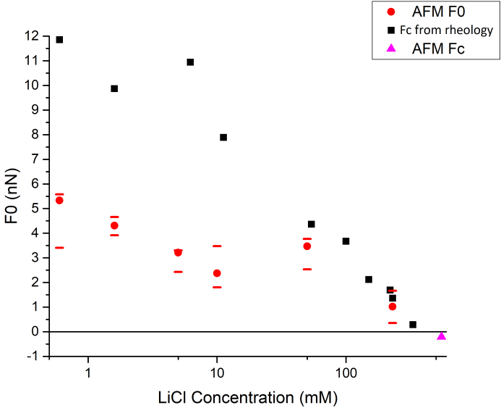
\includegraphics[width=0.45\textwidth]{chapter5/ContF1.png}\label{fig:CF1}}
  \hfill
  \subfloat[Site 2 curves.]{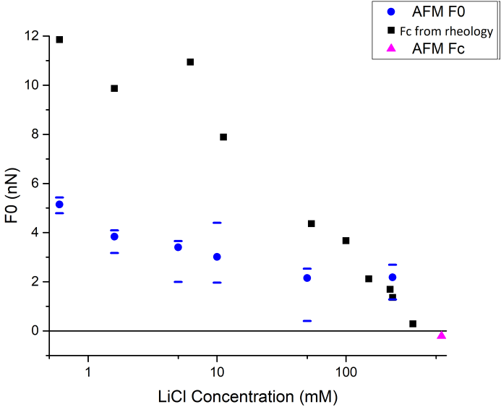
\includegraphics[width=0.45\textwidth]{chapter5/ContF2.png}\label{fig:CF2}}
  \caption{The resultant calculated repulsive force between the surface and the tip. The AFM data is compared against data taken from rheology. In the case of 550mM the repulsive forces transition to attractive, corresponding to the onset stress transitioning into yield stress (as seen from rheological data). F0 is taken from when the curve is within the onset of the contact region, Fc is taken from when the curve bends towards the surface, at the onset of contact (observable in \textit{Fig.3}. (a) and (b) are site 1 and 2 respectively\cite{John}.}
\end{figure}

\section{Shelf analysis}

The shelf seen in some datapoints is a consistent feature across multiple sites, present in the majority of the curves. The only concentration that doesn't feature the shelf in any of the sites is the 0.6mM concentrations, which is equally true in both the MFP and JPK AFMs.

However The shelf was also seen in the JPK forcemaps as well - specifically the 10mM curves. Though, the shelf prominence varies between sites, some have a visible shelf that extends across multiple nanometers, while others d

This feature is also seen in other papers from literature.\cite{guleryuz2012afm}

\section{Overcoming the noise in data}

The noise in the data from MFP AFM is significant. Not all AFMs can be operated in optimal conditions such as AFMs isolated from vibrations, under peak maintenance, free from external factors, etc. Other sources of noise in AFM can stem from electronic components, particularly those involved in the detection system, such as photodiodes and amplifiers. This includes shot noise from random electron motion, Johnson noise related to thermal motion within resistors, and noise intrinsic to operational amplifiers. Additionally, mechanical vibrations and thermal fluctuations also contribute to noise, affecting the spatial and temporal resolution of measurements. \cite{gittes1997signals}

Given the the MFP is potentially over 30 years old, these sources of noise could have impacted the resulting graphs from the age of the components in the system. In science there is a constant pressure to use newer equipment, when older equipment is still potentially suitable. Given that newer AFMs can brush up against the million pound mark, it is imperative to consider whether the trade-offs justify such investments. The challenge with older AFMs, particularly with models like the MFP, is that the wear and tear over time can exacerbate the inherent noise issues. Components such as piezoelectric scanners, which are responsible for the precise movements required for imaging and force measurements, may degrade in performance, leading to drifts or instability in the collected data. Similarly, older detection systems may not be as effective in filtering out noise or may not have the same sensitivity as modern instruments.

However, the core principles of AFM technology have remained consistent througout the years, the primary mechanisms of force detection and image resolution are still based on the deflection of a cantilever and the distance control between the probe and the sample. Hence, an older, well-maintained AFM can still provide valuable data, particularly for applications where ultra-high resolution is not mandatory.

The software developed during this investigation provides a powerful tool for older AFMs, particularly for noiser systems. The ability to resolve the shelf feature is a significant one, as the baseline noise present in the MFP curves often hide the feature. This capability is seen throughout all of the variability in conditions seen throughout the various different sites. By utilising the scripts and methods used in this investigation, it opens up the possibility of the scientific community to extend the lifespan of older equipment, making it viable for current and future research without the immediate need for costly upgrades.

The scripts and analysis methods developed as part of this research cater to the nuanced intricacies of noise in AFM data, enabling the extraction of meaningful results even from signals that might be considered too noisy or from data that would otherwise be discarded. This notion is particularly relevant in the context of educational institutions and research facilities with limited funding, where such software enhancements can democratize access to high-quality research opportunities. 

By making this software open source and accessible on a git repository, the scientific community can utilise, revise and improve upon tools that aloow for a greater applicability of AFM\cite{YourGithub2023}

may be due to the change in force applied to the surface. This is because the AFM is old and doesn't apply consistent pressure. It may have an affect, but you'd expect to see it more pronounced in the different salt concentrations. Plot the std dev vs concentration graph.

There is *alot* of noise at this scale. Because 
- I think it's cause it's a short period between phases?
- It's an old machine
- It hates me

Talk about how much noise there is. There is a lot of noise.

Show graphs

You can't just Lmao bin more cause then you have no data




Successful adaption and development of the glass treatment to AFM tips was performed. In particular a tip was treated with DCDMS surface coating. This tip was planned to be used with force mapping to investigate the presence of adhesive patches theorized by the group \cite{Teun1} and other literature \cite{Patchy}. 

\section{Tip speed}
Temporal Resolution of Electrostatic Forces: The speed at which the AFM tip approaches or retracts from the sample surface can affect the temporal resolution of the electrostatic forces. Faster tip speeds might not fully capture the gradual build-up or decay of electrostatic forces, whereas slower speeds allow for a more detailed measurement of these forces as they evolve over time. This is particularly important in systems where electrostatic interactions change rapidly with distance.

Dielectric Relaxation Effects: In systems where dielectric relaxation is significant, the speed of the AFM tip can impact how these relaxation processes are observed. Faster tip speeds may not allow enough time for the complete relaxation of the dielectric medium between the tip and the sample, leading to a different profile of electrostatic interaction compared to slower speeds.

Ion Mobility and Redistribution: In solutions with mobile ions, the movement of the AFM tip can cause redistribution of ions in the vicinity of the tip-sample interface. The speed of the tip can influence this redistribution, potentially altering the local ionic concentration and, consequently, the electrostatic interactions. Faster speeds might not allow sufficient time for ions to redistribute evenly, which could result in a different measurement compared to a scenario where the tip moves more slowly.

\section*{AFM contact force measurements and rheological behaviour of dense colloidal suspensions}

The significance of the present work does not confine in the direct measurement and fundamental understanding of forces of material surfaces in close proximity within aqueous media. Moreover, it allows us to investigate a working hypothesis in the colloidal rheology community regarding the onset of shear thickening behaviour in dense colloidal suspensions.~\cite{reference1}

Currently it is assumed that the colloidal particles do not experience any frictional forces at low shear stresses and it is only above an ``onset'' stress, $\sigma^*$, that frictional contact occurs leading to shear thickening behaviour.~\cite{reference2} It is speculated that it is this frictional contact occurring above the onset stress that is responsible for the characteristic viscosity increase observed during shear thickening. Following this reasoning, in order for the frictional contact to occur the shear stress has to overcome the repulsive interparticle force that inhibits contact, i.e. the repulsive critical “contact” force, $F_c$, which is directly related to the shear thickening onset stress $\sigma^*$. Using Derjaguin approximation [3], a critical surface energy $W^*$ can be associated with the critical force , $F_c$ (as measured by AFM) experiments as follows

% The formula can be included as follows
\[ W^*_{AFM} = \frac{F_c}{\pi R_t} \]

Where $W^*_{AFM}$ is the critical surface energy deduced from AFM fd curves and $R_t$ is the radius of the colloidal sphere we have used in these measurements ($3.3 \mu m$) at varying ionic strengths. The usage of the critical surface energy to describe the interactions has advantages as it is an intrinsic surface materials/media property and is independent of sizes. Equivalently, the shear thickening onset shear stress $\sigma^*$ in rheology experiments should also be related to this critical surface energy $W^*$ and simple dimensional analysis indicates that $W^* \propto R\sigma^*$, where $R$ is the radius of colloidal particles used in rheological experiments. More precisely, numerical simulations have already confirmed this relationship and provide the numerical predictor~\cite{reference4}.

\[ W^* = 2.11 R\sigma^* \]

Samuel C. Brown conducted systematic rheological experiments (colloidal silica spheres of radius of 0.75 μm) at different ionic strengths and a set of his measurements is used to calculate the critical surface energy in Figure \ref{fig:critical_surface_energy} where we also depict the calculated critical stress from the completely independent AFM fd curves presented in this thesis. The agreement is remarkable and indicates strongly and directly for first time the validity of the interparticle friction origins of the shear thickening behaviour.

% Here's how you might include a figure with a caption:
\begin{figure}[h!]
\centering
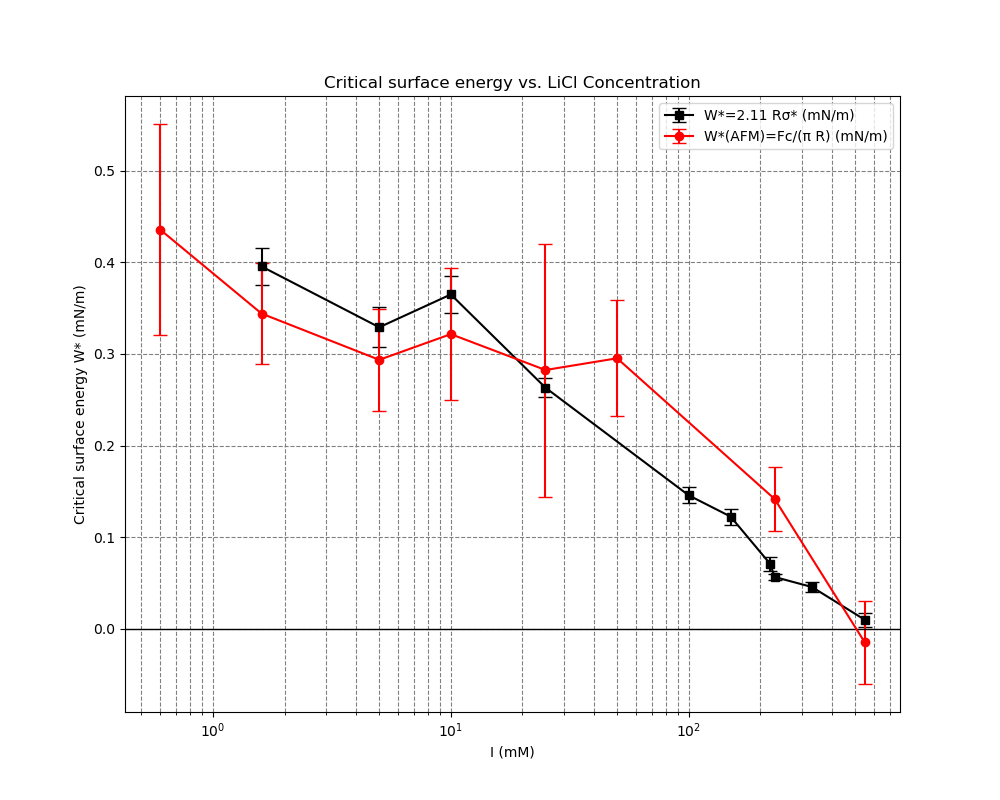
\includegraphics[width=\textwidth]{chapter8/Rheology/Comparison graph.png}
\caption{Critical surface energy values deduced from AFM (red circles) and rheological experiments (black squares) at different ionic strengths.}
\label{fig:critical_surface_energy}
\end{figure}

\section{Comparing results to DLVO theory}


The Force at Contact vs. LiCl Concentration plot is designed to show how the force at the point of contact between an Atomic Force Microscopy (AFM) tip and a sample varies with the concentration of LiCl in a 50:50 water-glycerol mixture. This relationship is important for understanding how ionic strength affects the interaction forces at the nanoscale.

\section*{Equations Used}

Several equations are used in the script to model the interactions. These equations are taken from chapter 1 to represent the types of equations used by those looking to model interactions. 

\textbf{Debye Length:} The inverse Debye length, $\kappa$, is given by
    \[
    \kappa = \sqrt{\frac{2 N_A e^2 I}{\varepsilon_0 \varepsilon_r k_B T}},
    \]
    where $N_A$ is Avogadro's number, $e$ is the elementary charge, $I$ is the ionic strength, $\varepsilon_0$ is the vacuum permittivity, $\varepsilon_r$ is the relative permittivity of the mixture, $k_B$ is the Boltzmann constant, and $T$ is the temperature. $\epsilon_r$ was taken from \cite{behrends2006dielectric}
    
\textbf{Electrostatic Repulsion Force:} The electrostatic repulsion force per unit area between a sphere and a plane, taking into account the surface potential $\Psi_0$, is calculated as
    \[
    U_E(r) = 2 \pi R \kappa \epsilon_0 \epsilon_r \left( \frac{k_B T}{e} \right)^2 \tanh^2\left(\frac{e \Psi_0}{4 k_B T}\right) e^{-\kappa h},
    \]
    where $R$ is the radius of the sphere and $h$ is the separation distance. $Psi_0$ was taken from \cite{silica2021}.
    
\textbf{Van der Waals Force:} The van der Waals force for a sphere-plane interaction is given by
    \[
    U_{\text{vdW}}(r) = -\frac{A_H R}{6 h^2},
    \]
    where $A_H$ is the Hamaker constant taken from \cite{Bergstrom1997}.
    
\textbf{Total Interaction Energy:} The total interaction energy or force at a separation $h$ is the sum of the van der Waals and electrostatic forces. When adjusted for surface roughness, the combined rms roughnesses of the two surfaces was added to the separation distance as a simple means to model roughness.


\section*{Plot Explanation}

The plot displays the calculated force at contact as a function of LiCl concentration. Experimental data points are overlaid to compare the theoretical model with actual measurements. The use of a logarithmic scale for the concentration axis allows for a clear visualization of the data over several orders of magnitude.

\begin{figure}[h!]
\centering
\includegraphics[width=\textwidth]{chapter8/cal}
\caption{Critical surface energy values deduced from AFM (red circles) and rheological experiments (black squares) at different ionic strengths.}
\label{fig:critical_surface_energy}
\end{figure}

\newpage
\newpage

\chapter{Conclusion}

